\documentclass{article}
\usepackage[utf8]{inputenc}
\usepackage{etoolbox}
\usepackage{hyperref}
\hypersetup{
    colorlinks=true,
    linkcolor=blue,
    filecolor=magenta,      
    urlcolor=cyan,
}

\urlstyle{same}
\usepackage{multicol}
\usepackage{graphicx}
\usepackage{wrapfig,lipsum}
\graphicspath{ {./images/} }

\usepackage{geometry}
 \geometry{
 a4paper,
 total={170mm,257mm},
 left=22mm,
 top=22mm,
 }

\usepackage{fancyvrb,newverbs,xcolor}
\definecolor{cverbbg}{gray}{0.93}

\newenvironment{cverbatim}
 {\SaveVerbatim{cverb}}
 {\endSaveVerbatim
  \flushleft\fboxrule=0pt\fboxsep=.5em
  \colorbox{cverbbg}{\BUseVerbatim{cverb}}%
  \endflushleft
}
\newenvironment{lcverbatim}
 {\SaveVerbatim{cverb}}
 {\endSaveVerbatim
  \flushleft\fboxrule=0pt\fboxsep=.5em
  \colorbox{cverbbg}{%
    \makebox[\dimexpr\linewidth-2\fboxsep][l]{\BUseVerbatim{cverb}}%
  }
  \endflushleft
}

\newcommand{\ctexttt}[1]{\colorbox{cverbbg}{\texttt{#1}}}
\newverbcommand{\cverb}
  {\setbox\verbbox\hbox\bgroup}
  {\egroup\colorbox{cverbbg}{\box\verbbox}}
  
\usepackage{titlesec}

\setcounter{secnumdepth}{4}

\titleformat{\paragraph}
{\normalfont\normalsize\bfseries}{\theparagraph}{1em}{}
\titlespacing*{\paragraph}
{0pt}{3.25ex plus 1ex minus .2ex}{1.5ex plus .2ex}
  

\begin{document}

\begin{center}
    \Large
    \textbf{The Letter Recognition from Sign Language Images}
\end{center}

\begin{flushleft}
\textbf{Student ID} 160709017
\newline\textbf{Name} Beyza
\newline\textbf{Surname} Kurt
\end{flushleft}

\begin{flushleft}

\section{Introduction}
"The Letter Recognition from Sign Language Images", the project I chose to do for the final project of the CENG 3521 Data Mining course, has been successfully completed and in this report, which models are suitable for images, which ones give better results and the cause-effect relationship between them are examined.

\section{TR Sign Language Dataset}
The data set is taken from \hyperlink{https://www.kaggle.com/berkaykocaoglu/tr-sign-language}{https://www.kaggle.com/berkaykocaoglu/tr-sign-language}.

\begin{itemize}
    \item There are no images of dotted or capped letters (i, ç, ş, ü, ö, ğ).
    \item It consists of 2 main folders as "train" and "test".
    \item There are at least 4000 photos for each letter in the "train" folder, and at least 1500 photos for those in the "test" folder.
    \item Apart from letters, there are 3 more folders named "del", "nothing" and "space" in "train" and "test" folders.
\end{itemize}

In the data set made ready for use in the project:

- "del", "nothing" and "space" folders have been removed.

- When it was understood that the program could not use all images due to lack of hardware, \textbf{the folders of each letter} in the "train" were moved to the main location with the first \textbf{2000} images. Thus, "train" and "test" files were removed and the data set in the code was divided into "train" and "test".

\vspace{2mm}
Figure~\ref{fig:tr_sign_language} below shows the sign language representation of all letters:

\begin{figure}[h]
    \centering
    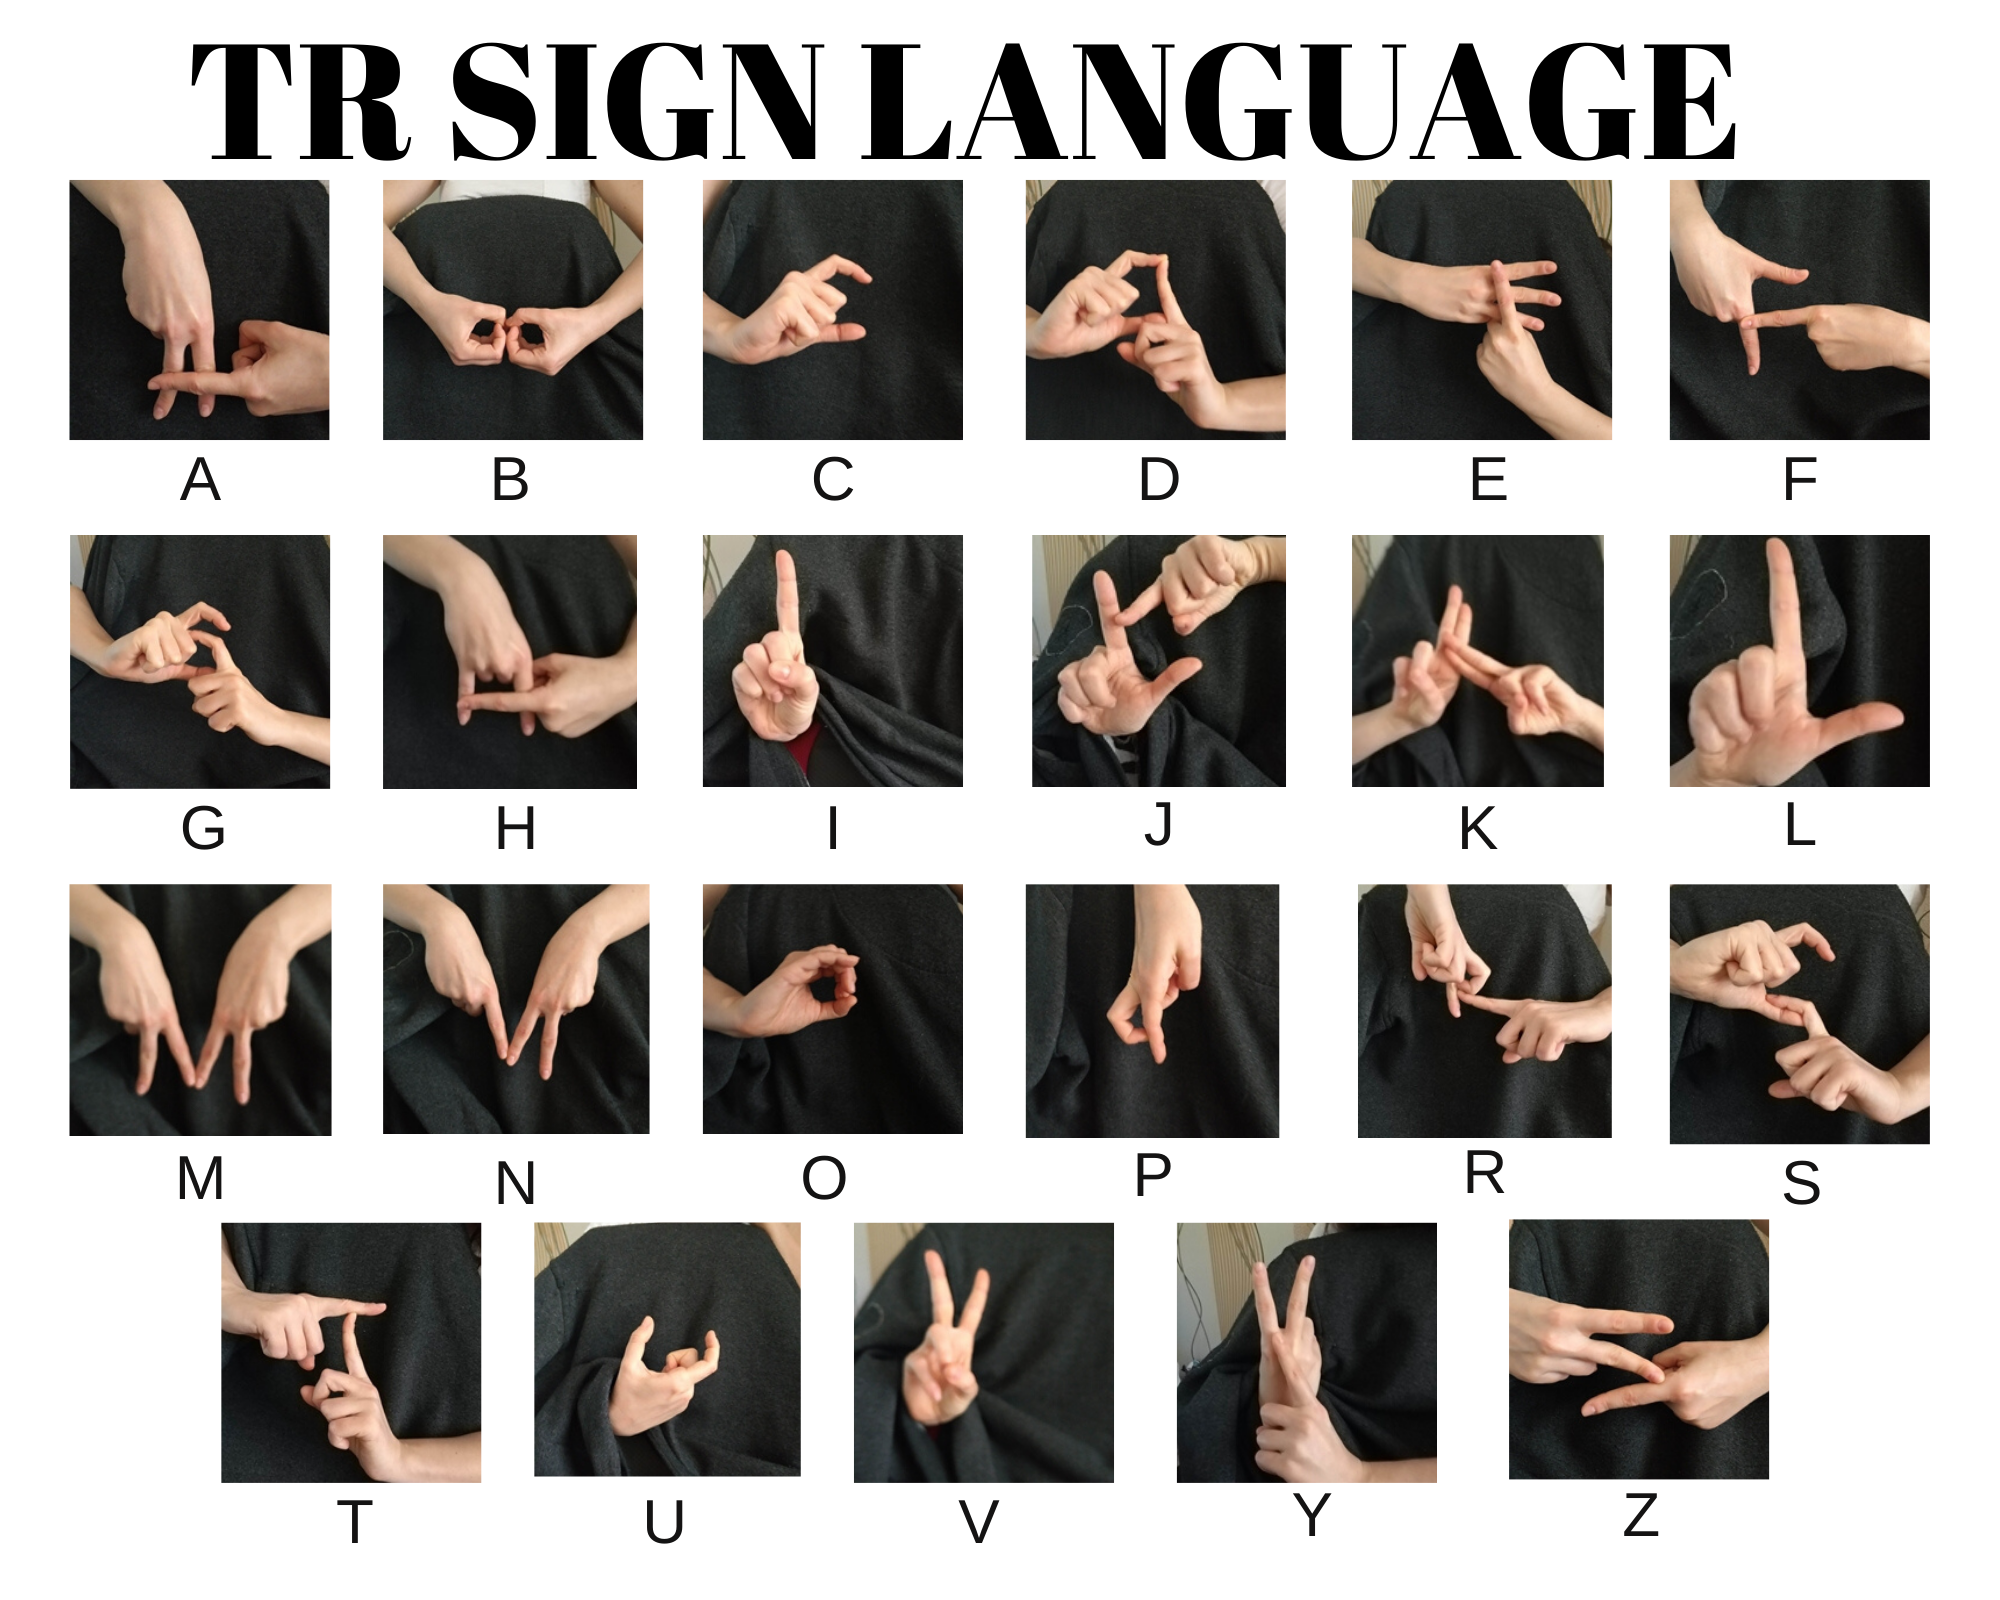
\includegraphics[scale=0.25]{images/tr sign language.png}
    \caption{TR Sign Language Images}
    \label{fig:tr_sign_language}
\end{figure}
\newpage

\section{Subjects}
\label{subjects}
Although I use images as data, instead of using libraries like keras that come to mind when it comes to "image classification", I wanted to put forward a study by sticking to the sklearn library we use in our homework. Because the digit data set we used during our homework was also a visual data set. I aimed to measure Sklearn's performance on another visual dataset.

\subsection{Data Preprocessing}
Because the images were colorful, they can be 3-dimensional arrays. This was not a suitable form to fit into classification models. Therefore, the rgb2gray function of skimage.color has been applied to all images. So they are grayscale and 2-dimensional now.

\vspace{2mm}
The states of an image whose original is not square, before and after the transformations are applied can be seen in Figure~\ref{fig:transformed_A}:

\begin{figure}[h]
    \centering
    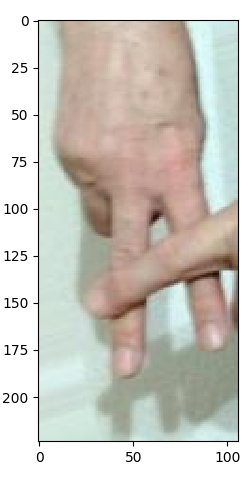
\includegraphics[scale=0.5]{images/A_original_2.png}
    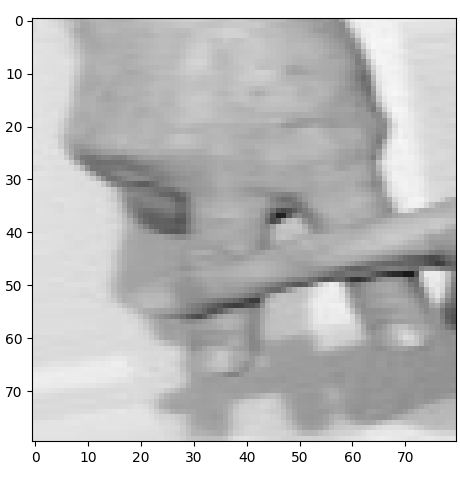
\includegraphics[scale=0.5]{images/A_transformed_2.png}
    \caption{An Image from Data Set; Before and After Transformation}
    \label{fig:transformed_A}
\end{figure}

I saved the images that are still not in proper form for the models by bringing them to a one-dimensional form using reshape().

Apart from these, I have examined how the following methods create effects on visuals, but I did not use them. The methods can be found in Section~\ref{methods} with sample visuals.

\subsubsection{Methods for Image Segmentation}
\label{methods}

\paragraph{Structural Similarity Index}
\begin{figure}[h]
    \centering
    \vspace{-5mm}
    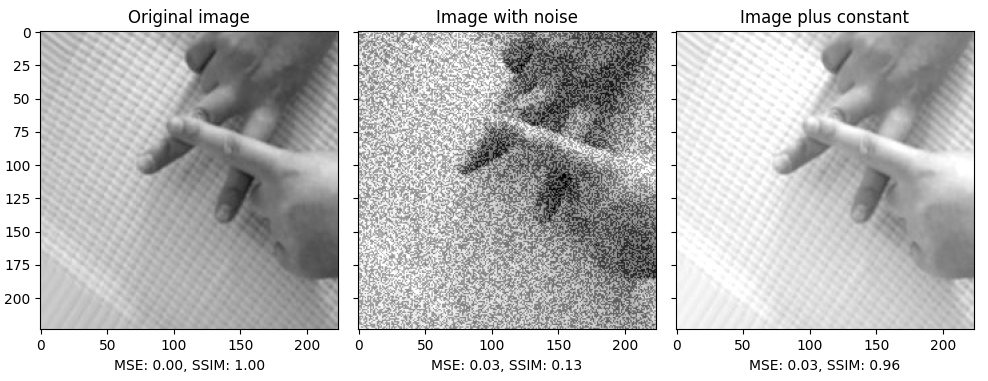
\includegraphics[scale=0.4]{images/structural_similarity_index.png}
    \caption{Structural Similarity Index}
    \label{fig:structural_similarity_index}
\end{figure}

The explanation of "Structural similarity index" in Scikit-Image documentation is as follows:

``When comparing images, the mean squared error (MSE)–while simple to implement–is not highly indicative of perceived similarity. Structural similarity aims to address this shortcoming by taking texture into account. The example shows two modifications of the input image, each with the same MSE, but with very different mean structural similarity indices.''

In one of the previous assignments, we added noise to the Digit dataset, but the form with no added noise performed best.


\paragraph{Thresholding}
\begin{figure}[h]
    \centering
    \vspace{-5mm}
    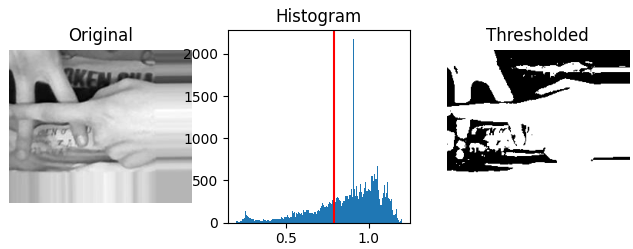
\includegraphics[scale=0.6]{images/thresholding.png}
    \caption{Thresholding}
    \label{fig:thresholding}
\end{figure}

The explanation of "Thresholding" in Scikit-Image documentation is as follows:

``Thresholding is used to create a binary image from a grayscale image. We illustrate how to apply one of these thresholding algorithms. Otsu’s method 2 calculates an “optimal” threshold (marked by a red line in the histogram below) by maximizing the variance between two classes of pixels, which are separated by the threshold. Equivalently, this threshold minimizes the intra-class variance.''

Although it might seem like it could achieve better results in this image, it was not used because it made most images meaningless.

\paragraph{Morphological Snakes}
\begin{figure}[h]
    \centering
    \vspace{-5mm}
    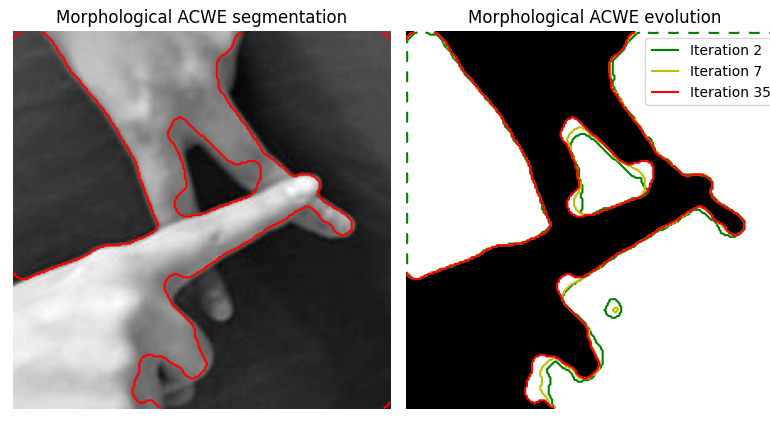
\includegraphics[scale=0.5]{images/morphological_snakes.png}
    \caption{Morphological Snakes}
    \label{fig:morphological_snakes}
\end{figure}

The explanation of "Morphological Snakes" in Scikit-Image documentation is as follows:

``Morphological Snakes use morphological operators (such as dilation or erosion) over a binary array instead of solving PDEs over a floating point array, which is the standard approach for active contours. This makes Morphological Snakes faster and numerically more stable than their traditional counterpart.''

Although it might seem like it could achieve better results in this image, it was not used because it made most images meaningless.


\subsection{Logistic Regression}
It is obvious that a linear classification method will not be effective for a visual data set. However, I still wanted to examine the results of my project by including linear models.In this direction, I used sklearn's linear models "LogisticRegression" and "SGDClassifier". You can see the results I have obtained using these two models, whose performances are almost the same, in Table x.

\begin{table}[h]
    \centering
    \begin{tabular}{c|c|c}
    \hline
        Model & Number of Sample for Each Letter & Score \\
    \hline
        LogisticRegression & 500 & 0.058840579710144926 \\
        SGDClassifier & 500 & 0.049871421710671843 \\
    \hline
    \end{tabular}
    \caption{Results of The Logistic Regression Models}
    \label{tab:logistic_Regression}
\end{table}

I expected the results to be low, but I was a little surprised that it was so low. Then I decided to test it using sklearn's digit dataset. You can find the results and the evaluation of the differences in Section~\ref{testing_on_digits}.

\subsection{Neural Network-based Classification}
I thought sklearn's neural network model MLPClassifier would do better after linear models. But again I did not get the results I expected. You can see the results in Table~\ref{tab:neural_network}.

\begin{table}[h]
    \centering
    \begin{tabular}{c|c|c}
    \hline
        Number of Sample for Each Letter & Hidden Layer Sizes & Score \\
    \hline
        500 & 32, 16, 8, 4, 2 & 0.08492753623188405 \\
        500 & 64, 32, 16, 8, 4, 2 & 0.09014492753623188 \\
        500 & 128, 64, 32, 16, 8, 4, 2 & 0.03826086956521739 \\
        500 & 256, 128, 64, 32, 16, 8, 4, 2 & 0.03826086956521739 \\
        500 & 512, 256, 128, 64, 32, 16, 8, 4, 2 & 0.03826086956521739 \\
    \hline
    \end{tabular}
    \caption{Results of The Neural Network-based Classification Models}
    \label{tab:neural_network}
\end{table}

Looking at the results, we cannot say that the increase in the hidden layer sizes for this data set has a positive effect on the result.

I also tested this model with sklearn's digits dataset. You can find the results and the evaluation of the differences in Section~\ref{testing_on_digits}.

\subsection{Ensemble Learning-based Classification}
For Ensemble Learning I used both models of sklearn: "VotingClassifier", "BaggingClassifier".

\begin{itemize}
    \item For the Voting Classifier, I used MLP classifiers that I created and stored in the previous step.
    \item I created an MLP classifier with (32, 16, 8, 4, 2) hidden layer sizes and splitted it into 5 equal parts. For the Bagging Classifier, I used them.
\end{itemize}

You can see the scores of the Voting classifier, the Bagging classifier and the split MLP classifiers I created for use in the Bagging classifier in Table x.

\begin{table}[h]
    \centering
    \begin{tabular}{c|c|c}
    \hline
        Model & Number of Sample for Each Letter & Score \\
    \hline
         Voting Classifier & 500 & 0.14115942028985506 \\
         Bagging Classifier & 500 & 0.10492753623188406 \\
         MLP Classifier 1 & 500 & 0.06985507246376811  \\
         MLP Classifier 2 & 500 & 0.07594202898550724  \\
         MLP Classifier 3 & 500 & 0.08057971014492754  \\
         MLP Classifier 4 & 500 & 0.06898550724637681  \\
         MLP Classifier 5 & 500 & 0.09014492753623188  \\
    \hline
    \end{tabular}
    \caption{Results of The Ensemble Learning-based Classification Models}
    \label{tab:ensemble}
\end{table}

If we look at the results of the MLP classifiers on Table~\ref{tab:neural_network} we created in the previous step, we can say that the performance of the Voting classifier that has made classification using them is better.

If we look at the results of the MLP classifiers on Table~\ref{tab:ensemble}, we can say that the performance of the Bagging classifier that has made better classification using 5 estimators in the ensemble.

I also tested this models with sklearn's digits dataset. You can find the results and the evaluation of the differences in Section~\ref{testing_on_digits}.


\section{Testing and Comparing with a Different Data Set}
\label{testing_on_digits}

I was not satisfied with the results I got, and I used sklearn's digits dataset to examine the results, both to check the accuracy of the code and to compare the performance of my dataset with another dataset. You can see the results in Table~\ref{tab:digits}.

\newpage
\begin{table}[h]
    \centering
    \begin{tabular}{c|c|c|c|c}
    \hline
        Model & Score && Model & Score \\
    \hline
        Logistic Regression & 0.9648148148148148 && Voting Classifier & 0.6 \\
        SGD Classifier & 0.9351851851851852 && Bagging Classifier & 0.9277777777777778 \\
        MLP Classifier 1 & 0.85 &&         Bagging MLP Classifier 1 & 0.4537037037037037 \\
        MLP Classifier 2 & 0.34629629629629627 && Bagging MLP Classifier 2 & 0.8203703703703704 \\
        MLP Classifier 3 & 0.38333333333333336 && Bagging MLP Classifier 3 & 0.08703703703703704 \\
        MLP Classifier 4 & 0.6407407407407407 && Bagging MLP Classifier 4 & 0.3611111111111111 \\
        MLP Classifier 5 & 0.5777777777777777 && Bagging MLP Classifier 5 & 0.8055555555555556 \\
    \hline
    \end{tabular}
    \caption{Results of All Models on the Digits Dataset}
    \label{tab:digits}
\end{table}

If we compare the results in Table~\ref{tab:digits} with the results in Section~\ref{subjects}, we can see that there is a huge difference between them. But first of all, we can say that \textbf{there is no error} in the accuracy of the code.

If we compare the data sets;
\begin{itemize}
    \item While a digit image that in the Digits data set is 8x8 in size, the images in the TR Sign Language Images data set are mostly 224x224x3. Reducing the dimensions to 80x80 with preprocessing may have caused a loss of accuracy.
    \item Even after preprocessing, the size of the photos 10 times larger than the digits data set may have decreased the accuracy.
    \item While there are 10 classes in the Digits dataset, there are 23 classes in the TR Sign Language Images dataset. This may have significantly reduced the accuracy of the estimates in the classification.
\end{itemize}

\section{Conv2D with Keras}
\label{conv2d}
Even though I checked it with the Digits data set, I made some experiments by looking at all the important parameters of the models; but the results continued to come low. So I wondered if the problem was that the models were not suitable for images. Thus, under the guidance of the article at \hyperlink{https://www.machinecurve.com/index.php/2020/03/30/how-to-use-conv2d-with-keras/}{https://www.machinecurve.com/index.php/2020/03/30/how-to-use-conv2d-with-keras/}, first verify that the model works properly with the CIFAR-10 dataset used in the article. then I run the model by putting my dataset to the appropriate form and review the results. Also, I used the dataset by taking 500 samples from each letter because the performance of my computer was not sufficient before. But this time, I created and used my dataset using all the existing images, without any limitation.

\begin{lcverbatim}
Epoch 1/50 403/403 [==============================] - 977s 2s/step - 
    loss: 3.1379 - accuracy: 0.0418 - val_loss: 3.1357 - val_accuracy: 0.0441
Epoch 2/50 403/403 [==============================] - 910s 2s/step - 
    loss: 3.1354 - accuracy: 0.0475 - val_loss: 3.1359 - val_accuracy: 0.0425
Epoch 3/50 403/403 [==============================] - 907s 2s/step - 
    loss: 3.1352 - accuracy: 0.0479 - val_loss: 3.1359 - val_accuracy: 0.0425
Epoch 4/50 403/403 [==============================] - 933s 2s/step - 
    loss: 3.1355 - accuracy: 0.0450 - val_loss: 3.1360 - val_accuracy: 0.0425
Epoch 5/50 403/403 [==============================] - 921s 2s/step - 
    loss: 3.1353 - accuracy: 0.0447 - val_loss: 3.1360 - val_accuracy: 0.0425
Epoch 6/50 403/403 [==============================] - 914s 2s/step - 
    loss: 3.1353 - accuracy: 0.0482 - val_loss: 3.1361 - val_accuracy: 0.0425
Epoch 7/50 403/403 [==============================] - 914s 2s/step - 
    loss: 3.1353 - accuracy: 0.0456 - val_loss: 3.1361 - val_accuracy: 0.0425
Epoch 8/50 403/403 [==============================] - 930s 2s/step - 
    loss: 3.1354 - accuracy: 0.0420 - val_loss: 3.1360 - val_accuracy: 0.0425
Epoch 9/50 403/403 [==============================] - 913s 2s/step - 
    loss: 3.1352 - accuracy: 0.0432 - val_loss: 3.1360 - val_accuracy: 0.0425
Epoch 10/50 403/403 [==============================] - 924s 2s/step - 
    loss: 3.1356 - accuracy: 0.0441 - val_loss: 3.1361 - val_accuracy: 0.0425
\end{lcverbatim}

I wanted to experiment with 50 epoch. But in the 10th epocht, I noticed that the value accuracy did not change. I did not continue to run it as this is proof that the progressive score value as low as 0.04 will not change much.

\section{Results}
Models could not reach adequate accuracy levels with TR Sign Language Images data set. I think the main reason for this is the data set itself. Because when I tried even with a model suitable for pictures, the score was not different from what I got with the models I wrote. Before testing the dataset with Conv2D, I thought it had a big impact that I could not use all the pictures because the performance of my computer or the resources I could use was not sufficient. But if we look at the Section~\ref{conv2d}, we can see that this is not quite true.

\vspace{2mm}
In addition, the increase in total speed was not high even when I ran the code by importing the data from Google Drive via Google Colab due to the inadequate performance of my computer. In fact, the process of importing files from Drive took much longer than on the computer, slowing the process.

\vspace{2mm}
Apart from these, the accuracy of the score may have been reduced due to the presence of images of letters similar to representation.

\section{References}
\begin{itemize}
    \item \hyperlink{https://scikit-learn.org/stable/modules/generated/sklearn.linear_model.LogisticRegression.html#}{sklearn.linear\_model.LogisticRegression}
    \item \hyperlink{https://scikit-learn.org/stable/modules/generated/sklearn.linear_model.SGDClassifier.html#}{sklearn.linear\_model.SGDClassifier}
    \item \hyperlink{https://scikit-learn.org/stable/modules/generated/sklearn.neural_network.MLPClassifier.html}{sklearn.neural\_network.MLPClassifier}
    \item \hyperlink{https://scikit-learn.org/stable/modules/generated/sklearn.ensemble.VotingClassifier.html#}{sklearn.ensemble.VotingClassifier}
    \item \hyperlink{https://scikit-learn.org/stable/modules/generated/sklearn.ensemble.BaggingClassifier.html#}{sklearn.ensemble.BaggingClassifier}
    \item \hyperlink{https://scikit-learn.org/stable/modules/generated/sklearn.datasets.load_digits.html}{sklearn.datasets.load\_digits}
    \item \hyperlink{https://www.machinecurve.com/index.php/2020/03/30/how-to-use-conv2d-with-keras/}{How to use Conv2D with Keras?}
    \item \hyperlink{https://www.cs.toronto.edu/\%7Ekriz/cifar.html}{The CIFAR-10 dataset}
    

\end{itemize}

\end{flushleft}
\end{document}